\documentclass{article}
\usepackage{amsmath}
\usepackage{graphicx} % Required for inserting images
\usepackage{tikz}
\usetikzlibrary{automata, positioning, arrows}

\title{Homework 4}
\author{}
\date{Due Date: May 17th, 2023}

\begin{document}

\maketitle
\tikzset{
         ->,  % makes the edges directed
         >=stealth, % makes the arrow heads bold
         node distance=3cm, % specifies the minimum distance between two nodes. Change if necessary.
         every state/.style={thick, fill=gray!10}, % sets the properties for each ’state’ node
         initial text=$ $, % sets the text that appears on the start arrow
         }
\section{Design question}
Design a system using the publisher subscriber model , for the follow scenario - a robot displays a tennis ball in its visual field(camera) then navigates to the position of the tennis ball. Assume you are in a room where the only yellow object is the tennis ball.\\\\
\textbf{Solution: }\\
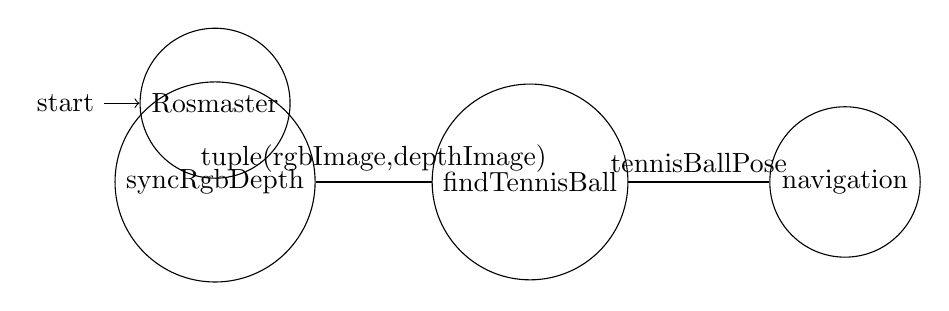
\begin{tikzpicture}
    % tikz code goes here
    \node[state, initial] (1) {Rosmaster};
    \node[state, below of=1] (2) {syncRgbDepth};
    \node[state, below of=1, right of=2] at (3,0) (3) {findTennisBall};
    \node[state, below of=1, right of=3] at (7,0) (4) {navigation};

    \draw   (2) edge[above] node{tuple(rgbImage,depthImage)} (3)
            (3) edge[above] node{tennisBallPose} (4);
\end{tikzpicture}
\label{fig:my_label}
\section{Programming question}
1. Use theconstructsim.com to develop a node that uses turtlesim to draw a hexagon with sides equal to 1. Do not hard code the points and instead try to use the geometric properties of the hexagon to draw the shape.\\
2. Given point ${}^AP_1= \begin{bmatrix} 2 \\1  \end{bmatrix}$ in the turtles frame, write a node that prints this point in the world frame(the map on simulator), run this node alongside part 1 of this question.\\\\

\textbf{SOLUTION for 1 and 2 ON BLACKBOARD hw4.py}
\end{document}
